\section{Introduction}

This is an era of big data, and IDC even estimated the exponential growth of data by a factor of 10 \cite{KouzesR2009_ChangingParadigm, SakrR2011_Survey}.
The growing data set provides huge potential for business and research to explore.
Thus, big data analytics has become critical demand to dig valuable information from explosive growing data.
The giant volume of data along with its variety and velocity poses great challenge to big data analytics\cite{PaulZik2011_UnderstandingBigData}, and therefore its optimization remains an active research domain.

The MapReduce programming model has gained increasing success for parallel data processing because of its horizontal scale and fault tolerance \cite{DeanJ2004_MapReduce}.
Apache Hadoop \cite{hadoop} and Microsoft Dryad \cite{IsardM2007_Dyrad}, for example, are popular systems that embrace this model.
In order to handle large-scale data, these systems usually run on top of large clusters of commodity machines and tightly couple computation and storage nodes.
This design enables a system to scale out easily because the ratio between computation power and I/O capability remains constant \cite{DeanJ2004_MapReduce, hadoop, BellG2006_Petascale}.

\begin{figure}[ht]
    \centering
    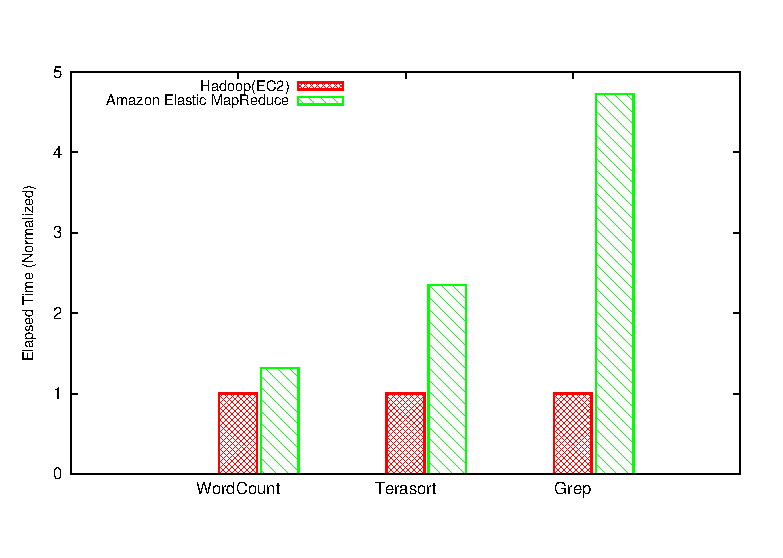
\includegraphics[width=0.8\textwidth]{figures/decoupled_performance.eps}
    \caption{Hadoop performance in the decoupled model.  Four x1.large instances are used, and Amazon EMR uses Amazon S3 as the storage for input and output files.  Amazon EMR does not utilize all available machines because its resource scheduler does not fit the decoupled Hadoop model.}
    \label{fig:decoupled_performance}
\end{figure}

However, this principle imposes a strong constraint on system design, and thus cannot apply to many use cases, such as enterprises application \cite{MihailescuM2012_MixApart, PorterG2010_SuperDataNodes}, scientific computing \cite{BresnahanJ2011_Cumulus, RamakrishnanL2010_EScience}, and cloud computing \cite{AWS, WindowsAzure, GoogleCloud}.
For example, storage area network (SAN) is popular in enterprise and Amazon Simple Storage Service (Amazon S3) is the recommended storage for Amazon web services.
These scenarios prefer a separate storage architecture because of high efficient storage, data lifecycle management and elastic cloud storage.
More importantly, this separate architecture provides high flexibility of system deployment, which is a big challenge in enterprise and datacenter management \cite{ShaferJ2010_PhD, PorterG2010_SuperDataNodes}.
For these reasons, we believe the decoupled model will become more important for MapReduce and Hadoop.

The decoupled mode has emerged but only few research studies pay attention to this scenario.
This situation leads to poor performance when running Hadoop with the decoupled model as shown in Figure \ref{fig:decoupled_performance}.
To understand the performance of the decoupled model, we ran three different types of jobs on Amazon EC2 for the Hadoop reference model and Amazon Elastic MapReduce for the decoupled one.
The result shows that the decoupled model has system throughput that is much lower than we expected.
We find that existing Hadoop schedulers cannot work well when data locality no longer exists.
Besides, we doubt that the overhead of large data movement can greatly affect system throughput because the storage system and the network infrastructure cannot fulfill the demand of Hadoop applications.

In this paper, we view the decoupled Hadoop model as a flow network in which data flows through computation and storage facilities.
The data flow rate is the amount of data  processed or transferred per unit of time, and the system throughput can be measured by the flow rate.
We argue that maintaing high data flow rate can increase the system throughput.
In the decoupled model, there are two possible conditions that a computation facility does not fully utilize its processing power:
1) the flow rate of data supply from the remote storage facility is not fast enough and
2) the computing facility cannot process data flow fast enough.
The first case can happen when the storage facility cannot handle a large number of simultaneous data access and when network infrastructure cannot sustain such a large amount of data transfer, especially when cross-rack communication happens.
The second case comes from the overhead of operating system and the data access over network.
We believe eliminating undesired factors that affects the processing flow rate can increase the system throughput in the meanwhile.

We propose a flow scheduling method that models the penalty cost of task assignments.
Given the cost model, we encode the scheduling problem as the min-cost flow problem so that we can derive the optimal task assignment.
We have designed Hadoop Flow Scheduler that implements our flow scheduling method.
This Flow Scheduler requires job profile and machine profile in order to decide the optimal task assignment.
We first estimate the flow demand of tasks and the flow capability of facilities and then feed this information to our Flow Scheduler.
Our experiment result shows that we can improve the system throughput by up to 30\%.
More importantly, our flow scheduling method can eliminate stragglers in the decoupled model and provide more smooth task execution time.

This paper is organized as follows.
Section \ref{sec:background} provides the background on the new Hadoop design and the decoupled model.
Section \ref{sec:flow_scheduling} describes the ideal behind our flow scheduling method, the definition of data flow rate and the cost model for task assignment.
Section \ref{sec:flow_scheduler} details the Flow Scheduler implantation for Hadoop and how we estimate the data flow rate.
We evaluate Flow Scheduler in  Section \ref{sec:evaluation} and discuss the limitation of current implementation.
Section \ref{sec:related_work} gives the most related work and we conclude in Section \ref{sec:conclusion}.
